\documentclass[a4paper,12pt,luatex]{ltjsarticle}
\usepackage[hiresbb]{graphicx}
\usepackage{booktabs}
\usepackage[table]{xcolor}
\usepackage{float}
\usepackage{subcaption}
\usepackage[backend=biber, style=numeric]{biblatex}
\addbibresource{myrefs.bib}

\begin{document}

文献を参照する方法については van Leunen~\cite{leunen},木下~\cite[pp.\,161--167]{木下:作技}
が参考になろう。

% \bibliographystyle{jplain}
% \bibliography{myrefs}
\printbibliography[title=参考文献]
\end{document}
% SPA \part{}
% SCH \chapter{}
% \section{図の配置}
% SSS \subsection{}
% SS2 \subsubsection{

% \subsection{図の罫線について}

% \begin{center}
%     \begin{tabular}{lrr} \toprule
%         items   & units & num \\ \cmidrule(lr){1-3}
%         apple  & 100       & 5 \\
%         orange  & 50        & 10\\ \bottomrule
%     \end{tabular}
% \end{center}

% \subsection{図の彩色}

% \begin{center}
%     \begin{tabular}{|>{\columncolor[gray]{0.8}}c|c|} \hline
%         1列目 line & 2nd line \\ \hline
%         1st line & 2nd line \\ \hline
%     \end{tabular}
% \end{center}

% \subsection{表のキャプションと桁揃え}

% 表\ref{hyou}にキャプション付きの表を示す。

% \begin{table}[b]
% \caption[caption]{table No.1}
% \label{hyou}
%     \begin{center}
%         \renewcommand{~}{\phantom{0}}

%         \begin{tabular}{rlr}                                        \toprule
%             \multicolumn{1}{c}{$T$ (deg)} &
%             \multicolumn{1}{c}{$t$ (sec)} &
%             \multicolumn{1}{c}{$X_n$}                               \\ \midrule
%             $ 10^{12}$              & ~0            & 0.496         \\[-4pt]
%             $ 3 \times 10^{11}$     & ~0.001129     & 0.488\rlap{*} \\[-4pt]
%             $ 1.3 \times 10^{9~}$   & 98*           & 0.15~         \\ \bottomrule
%         \end{tabular}
%     \end{center}
% \end{table}

% \clearpage

\section{図の配置}

% 図\ref{fig:trump}にトランプ大統領を示す。

% \begin{figure}[h]
%     \centering
%     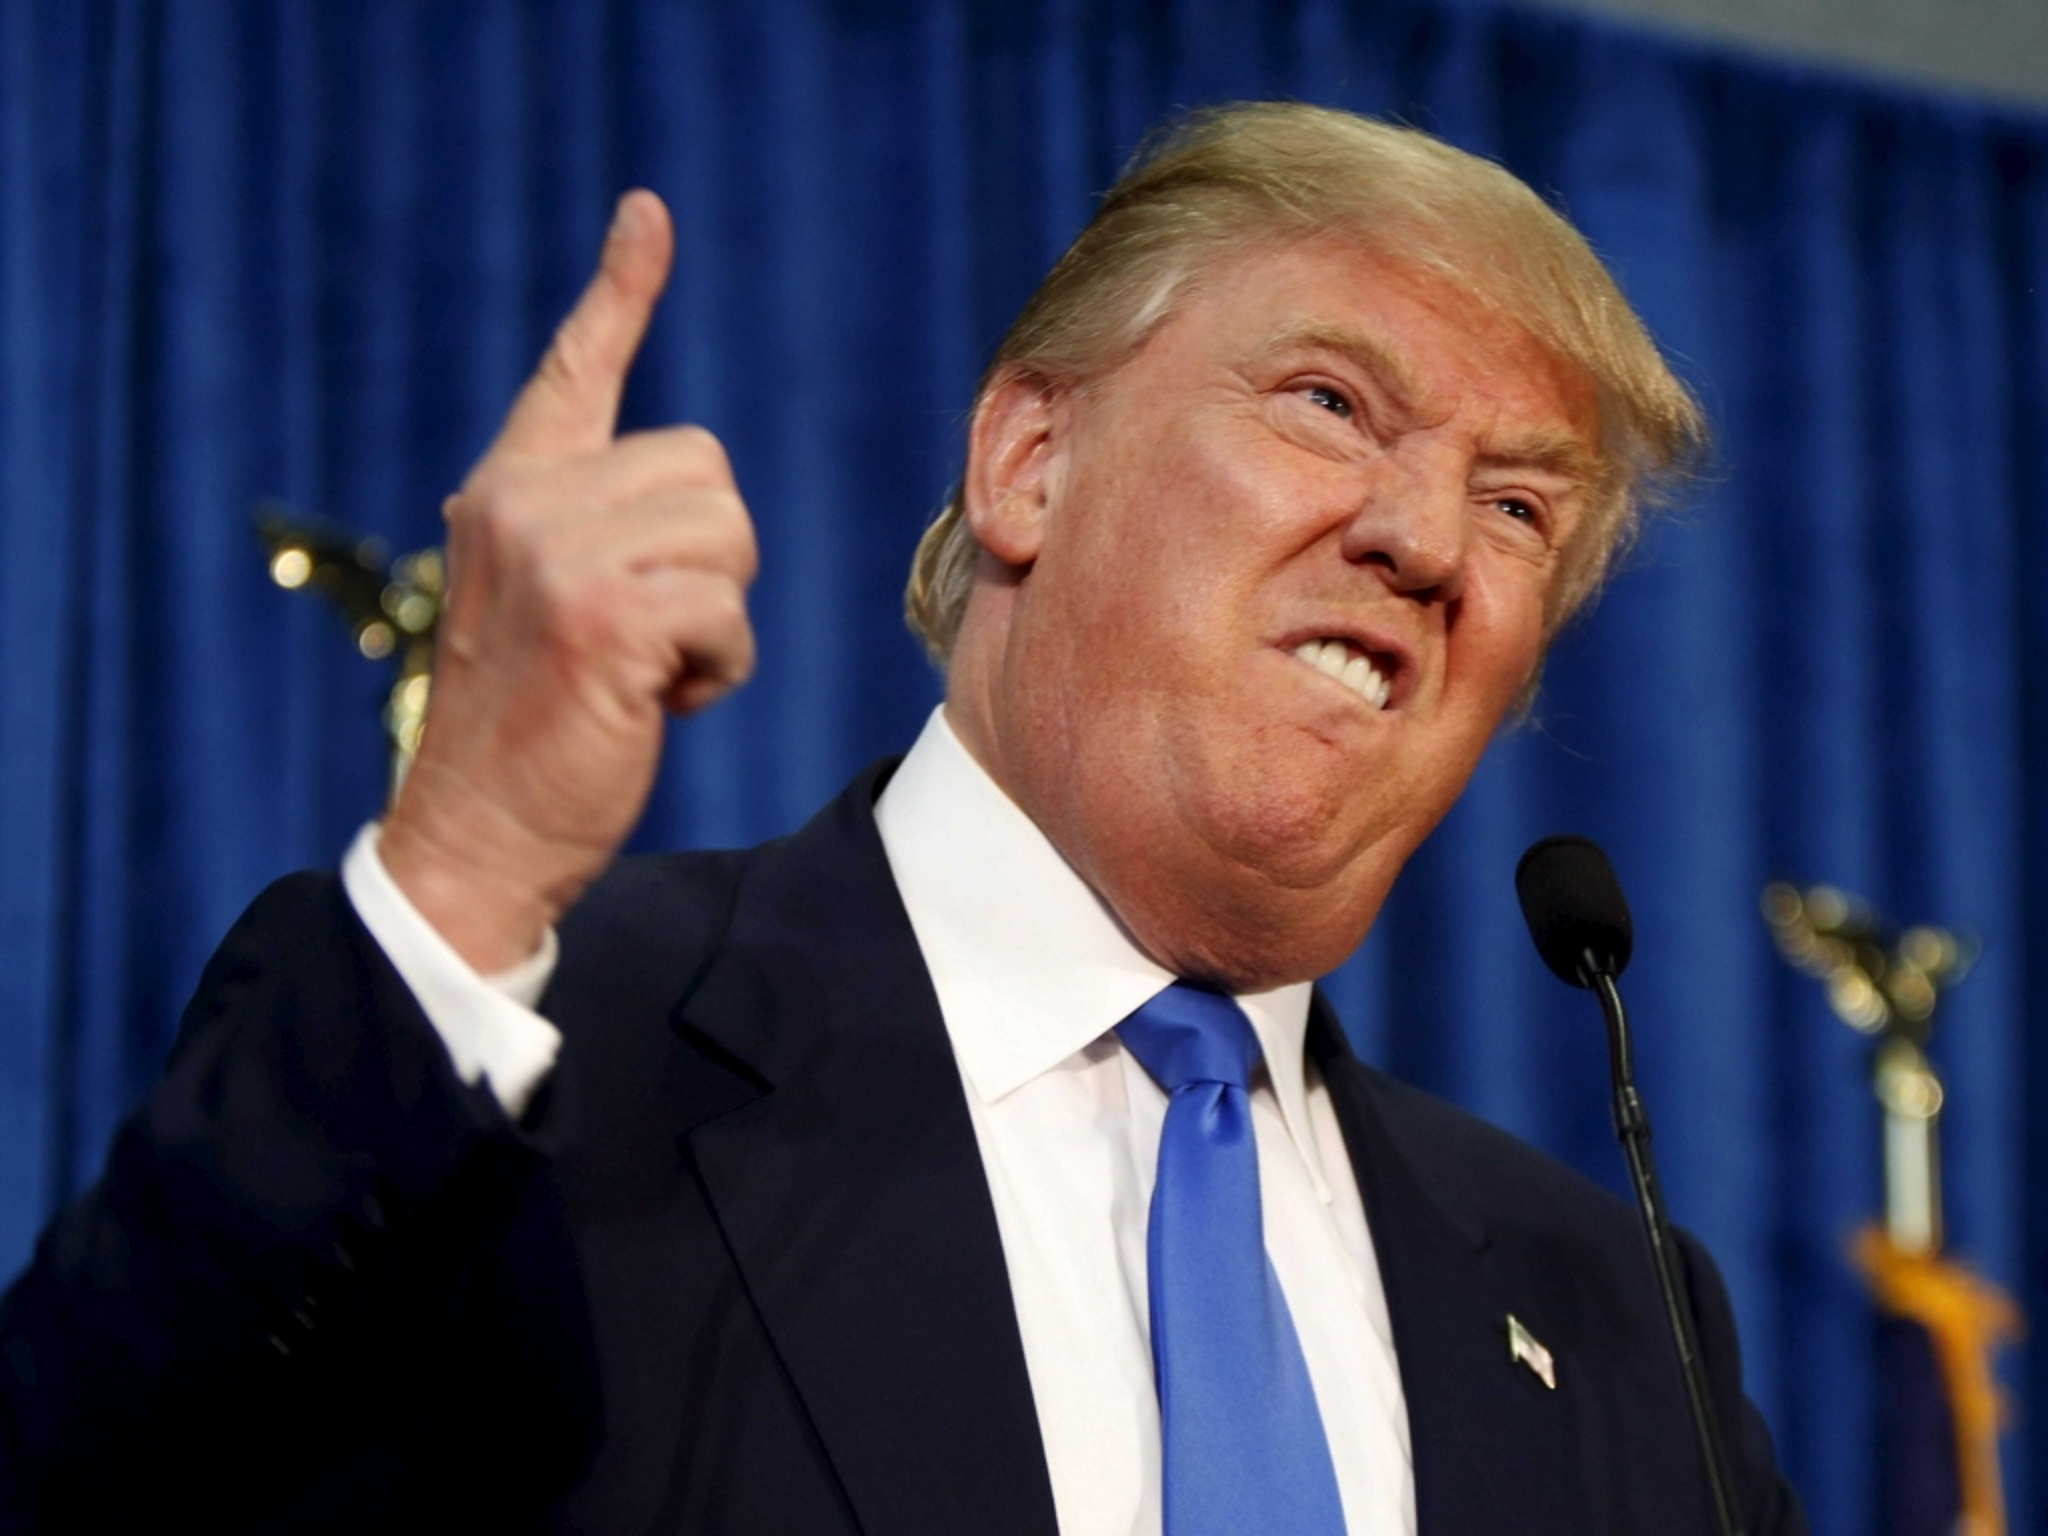
\includegraphics[width=8cm, draft]{trump01.jpg}
%     \caption{トランプ大統領}
%     \label{fig:trump}
% \end{figure}

% 関連した複数の図を並べるには...
% \begin{figure}[ht]
%     \centering
%     % 右の図
%     \begin{minipage}{0.4\columnwidth}
%         \centering
%         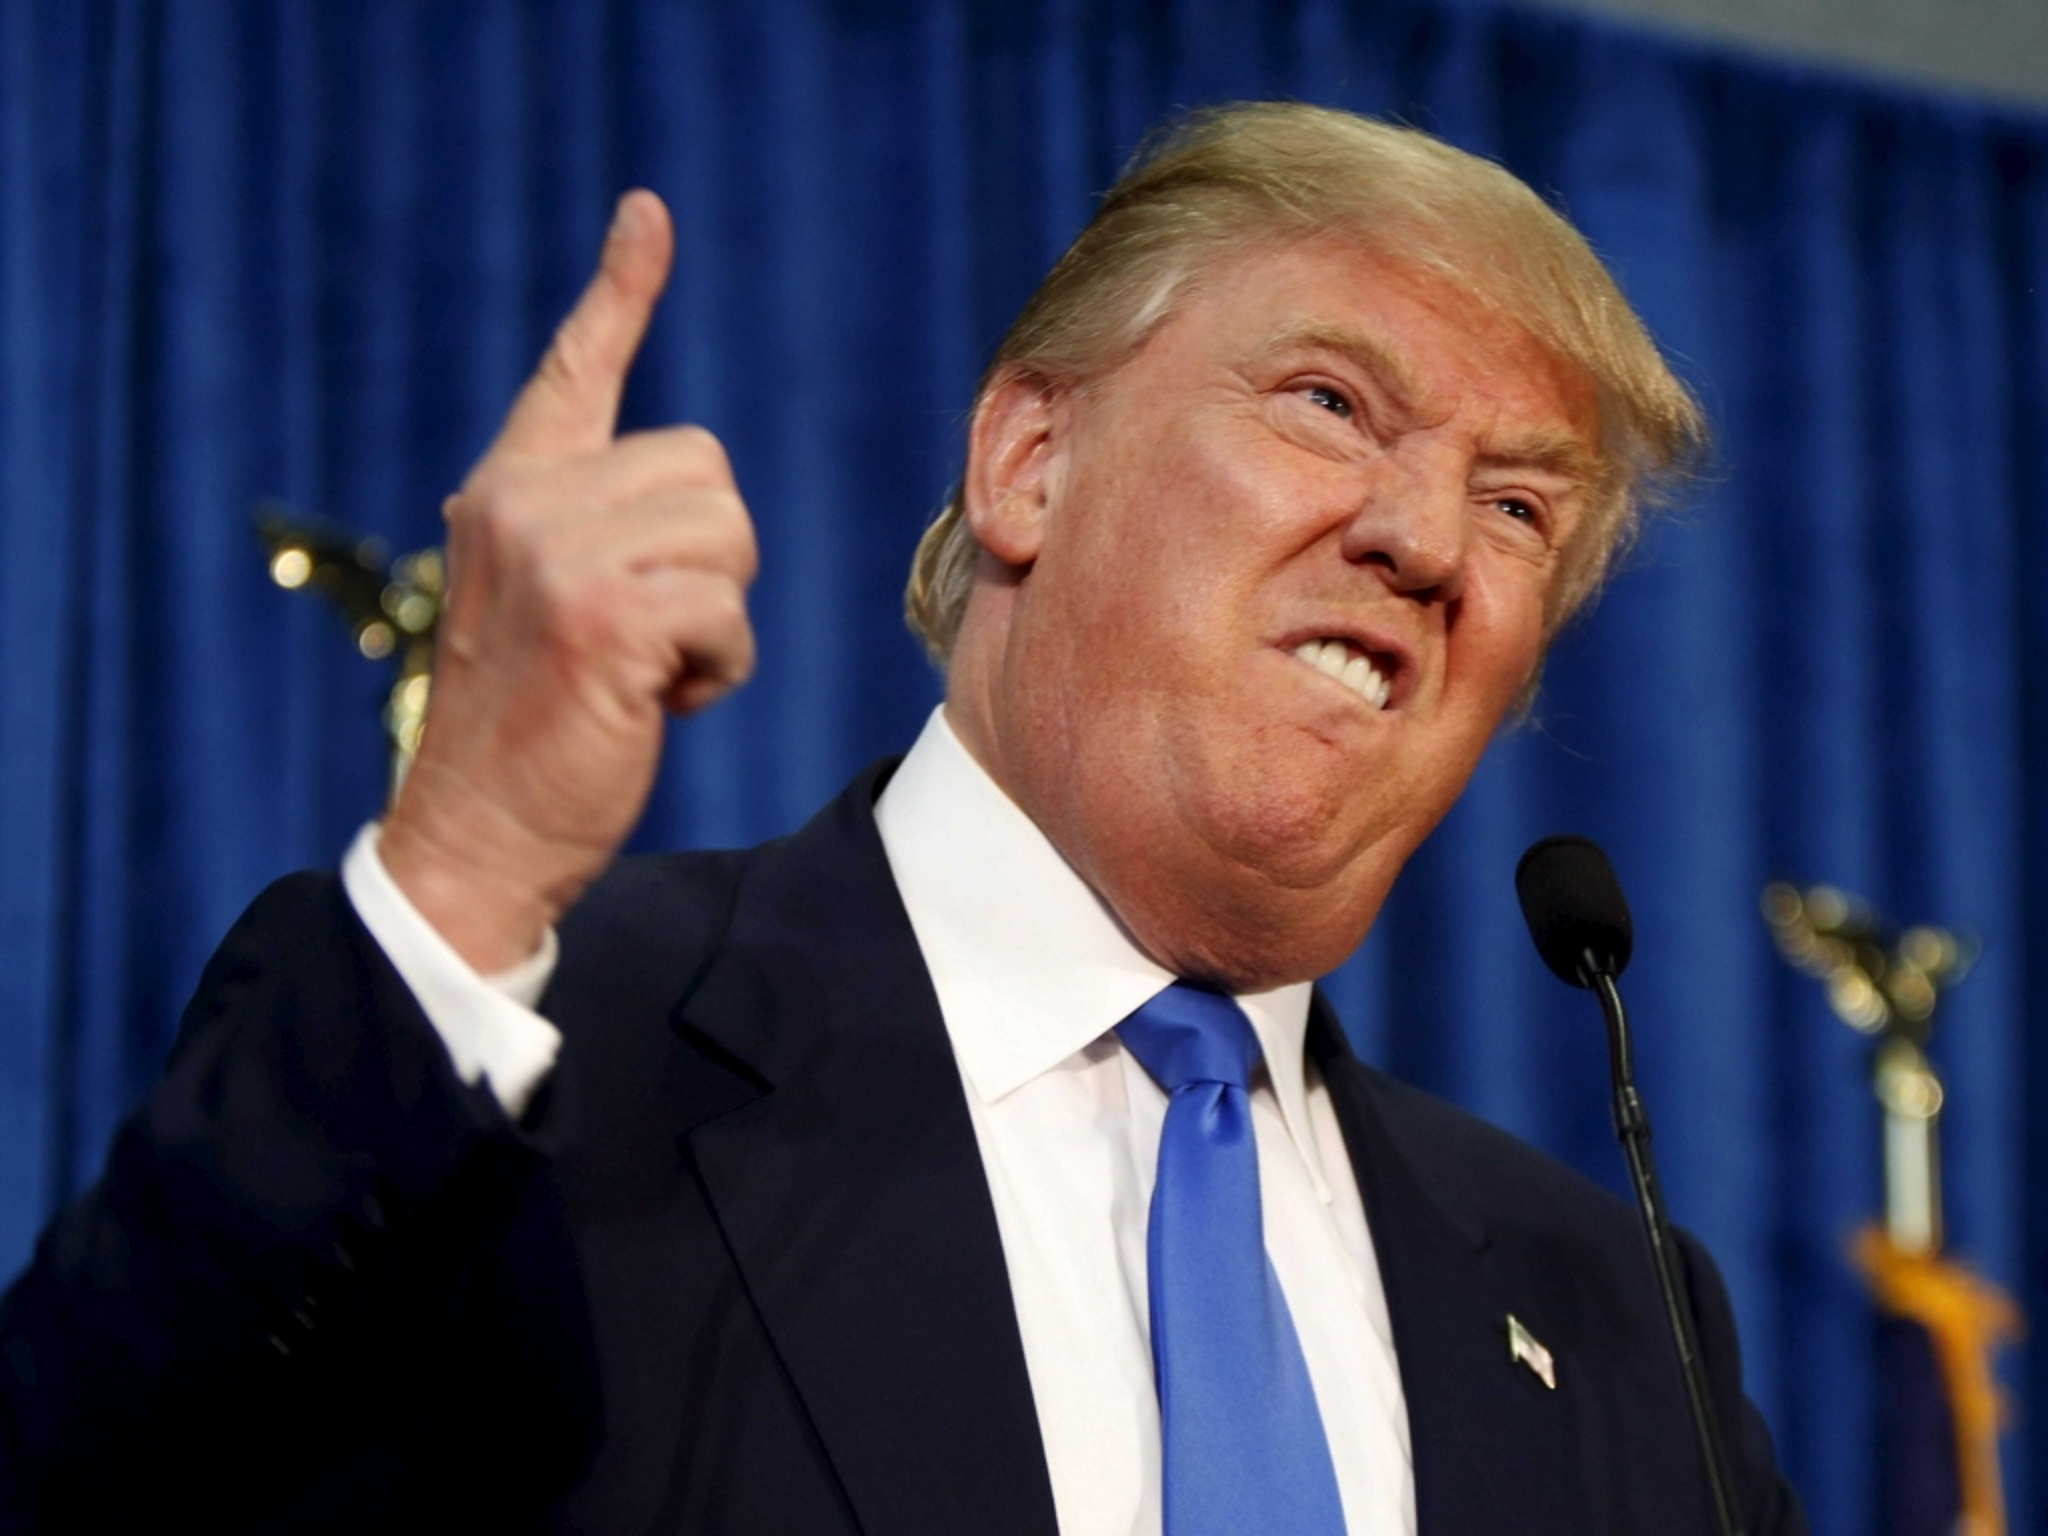
\includegraphics[width=\columnwidth]{trump01.jpg}
%         \caption{左の図}
%         \label{fig:left}
%     \end{minipage}
%     % 左の図
%     \begin{minipage}{0.4\columnwidth}
%         \centering
%         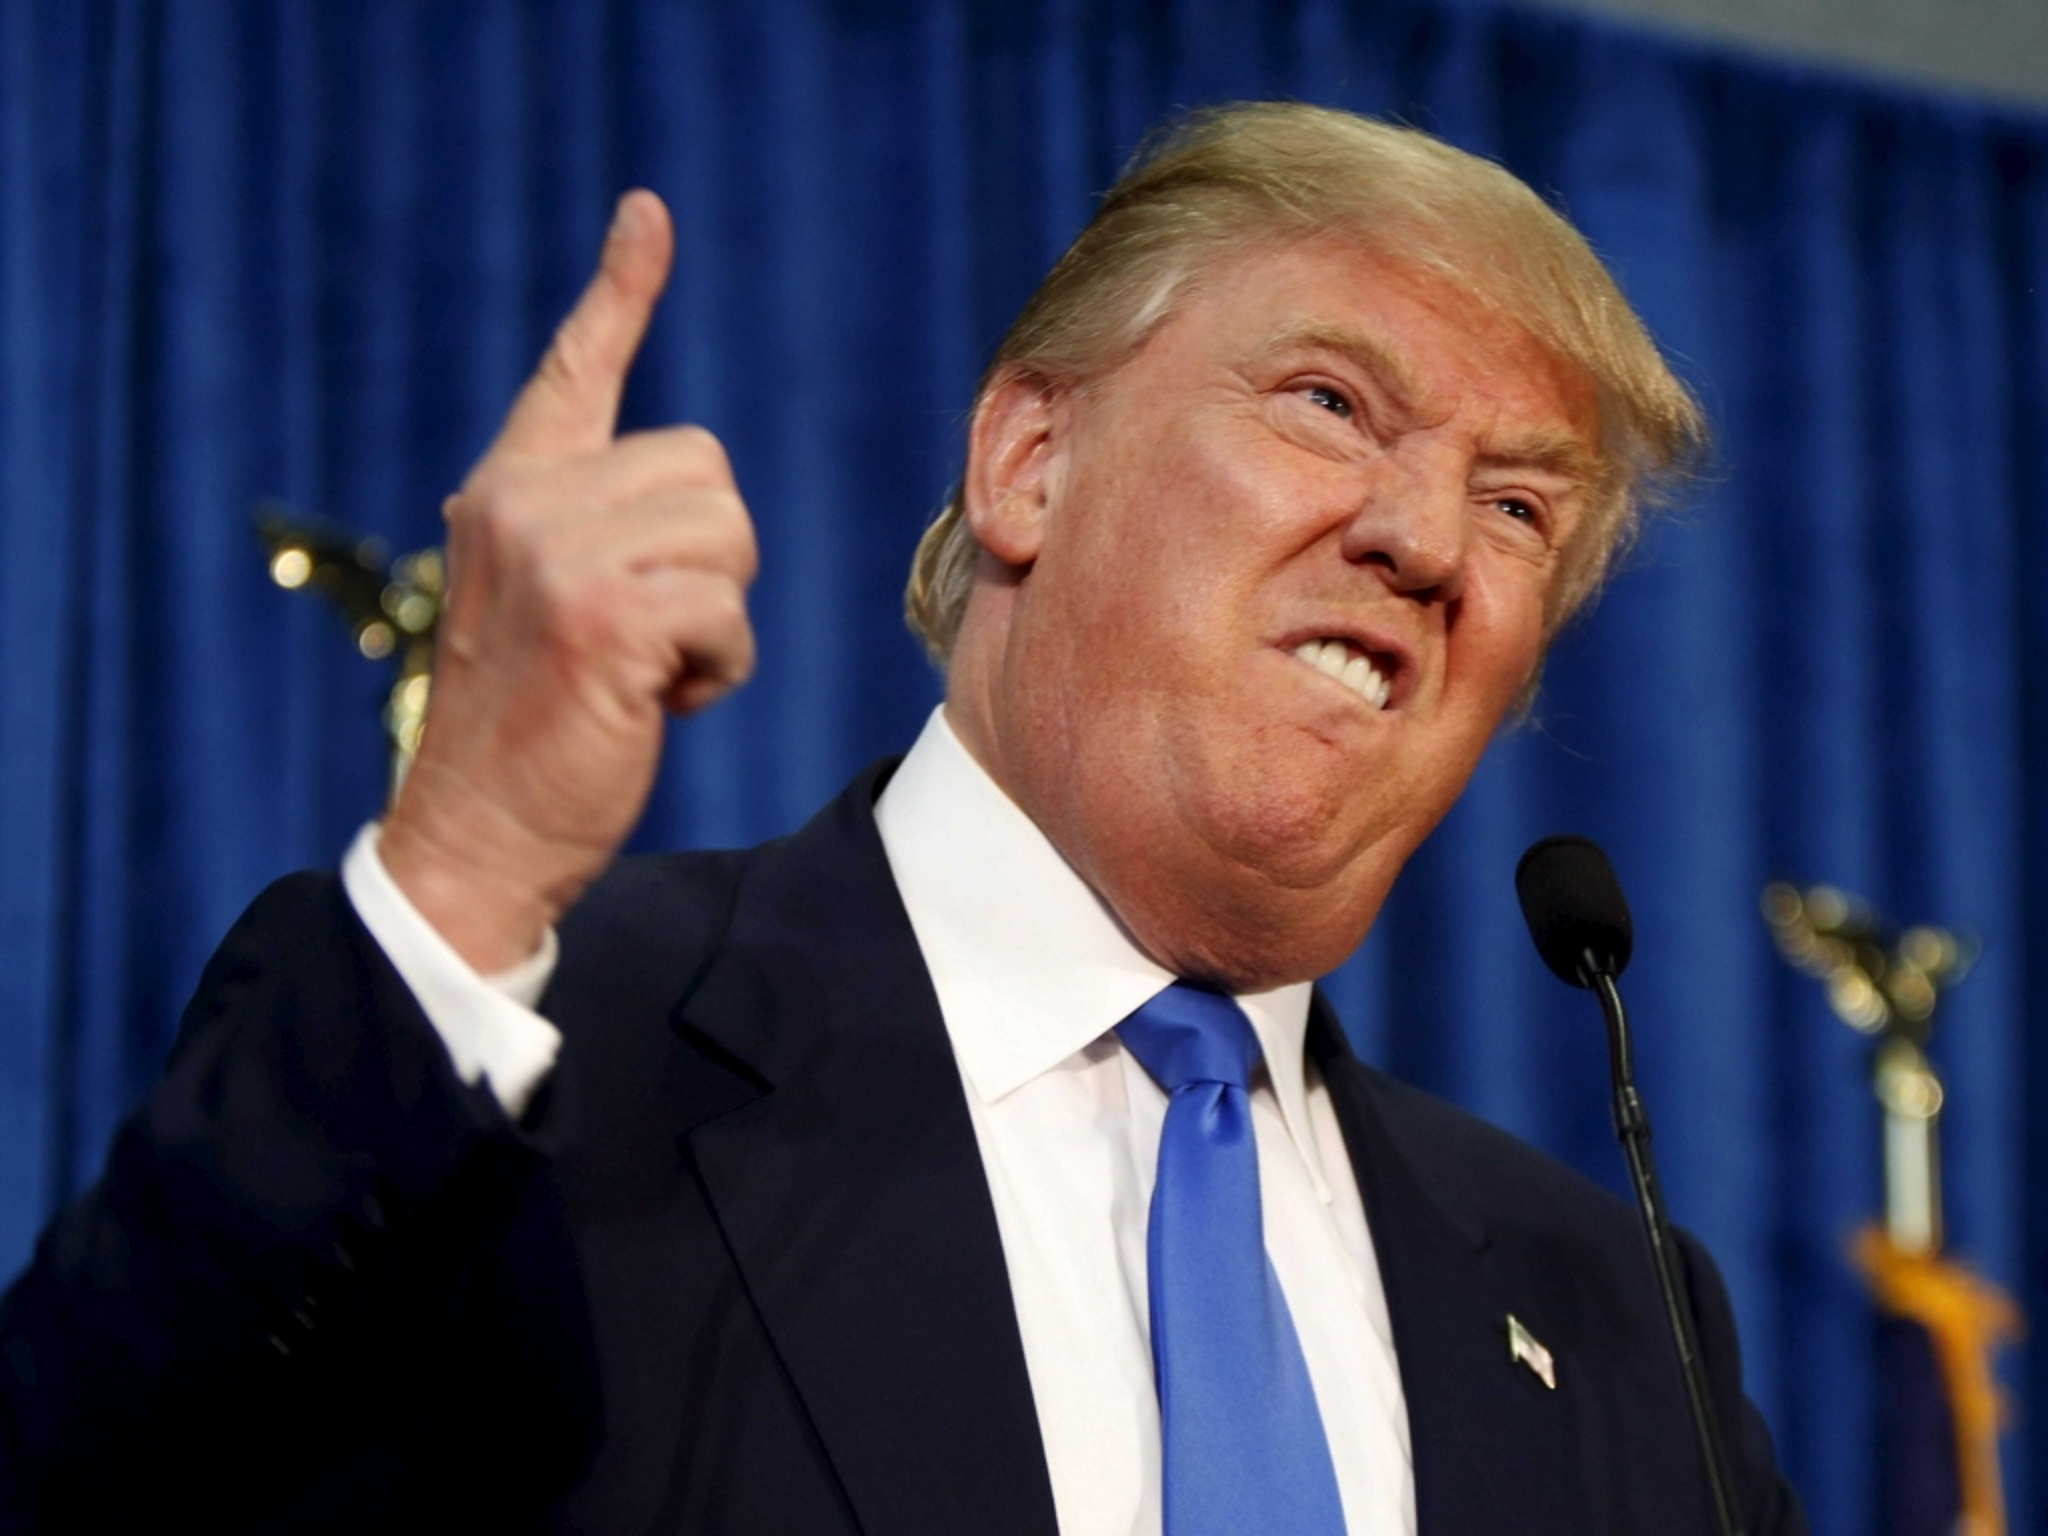
\includegraphics[width=\columnwidth]{trump01.jpg}
%         \caption{右の図}
%         \label{fig:right}
%     \end{minipage}
% \end{figure}

% 関連した複数の図を並べるには...

% \begin{figure}[ht]
%     \centering
%     % 右の図
%     \begin{subfigure}{0.4\columnwidth}
%         \centering
%         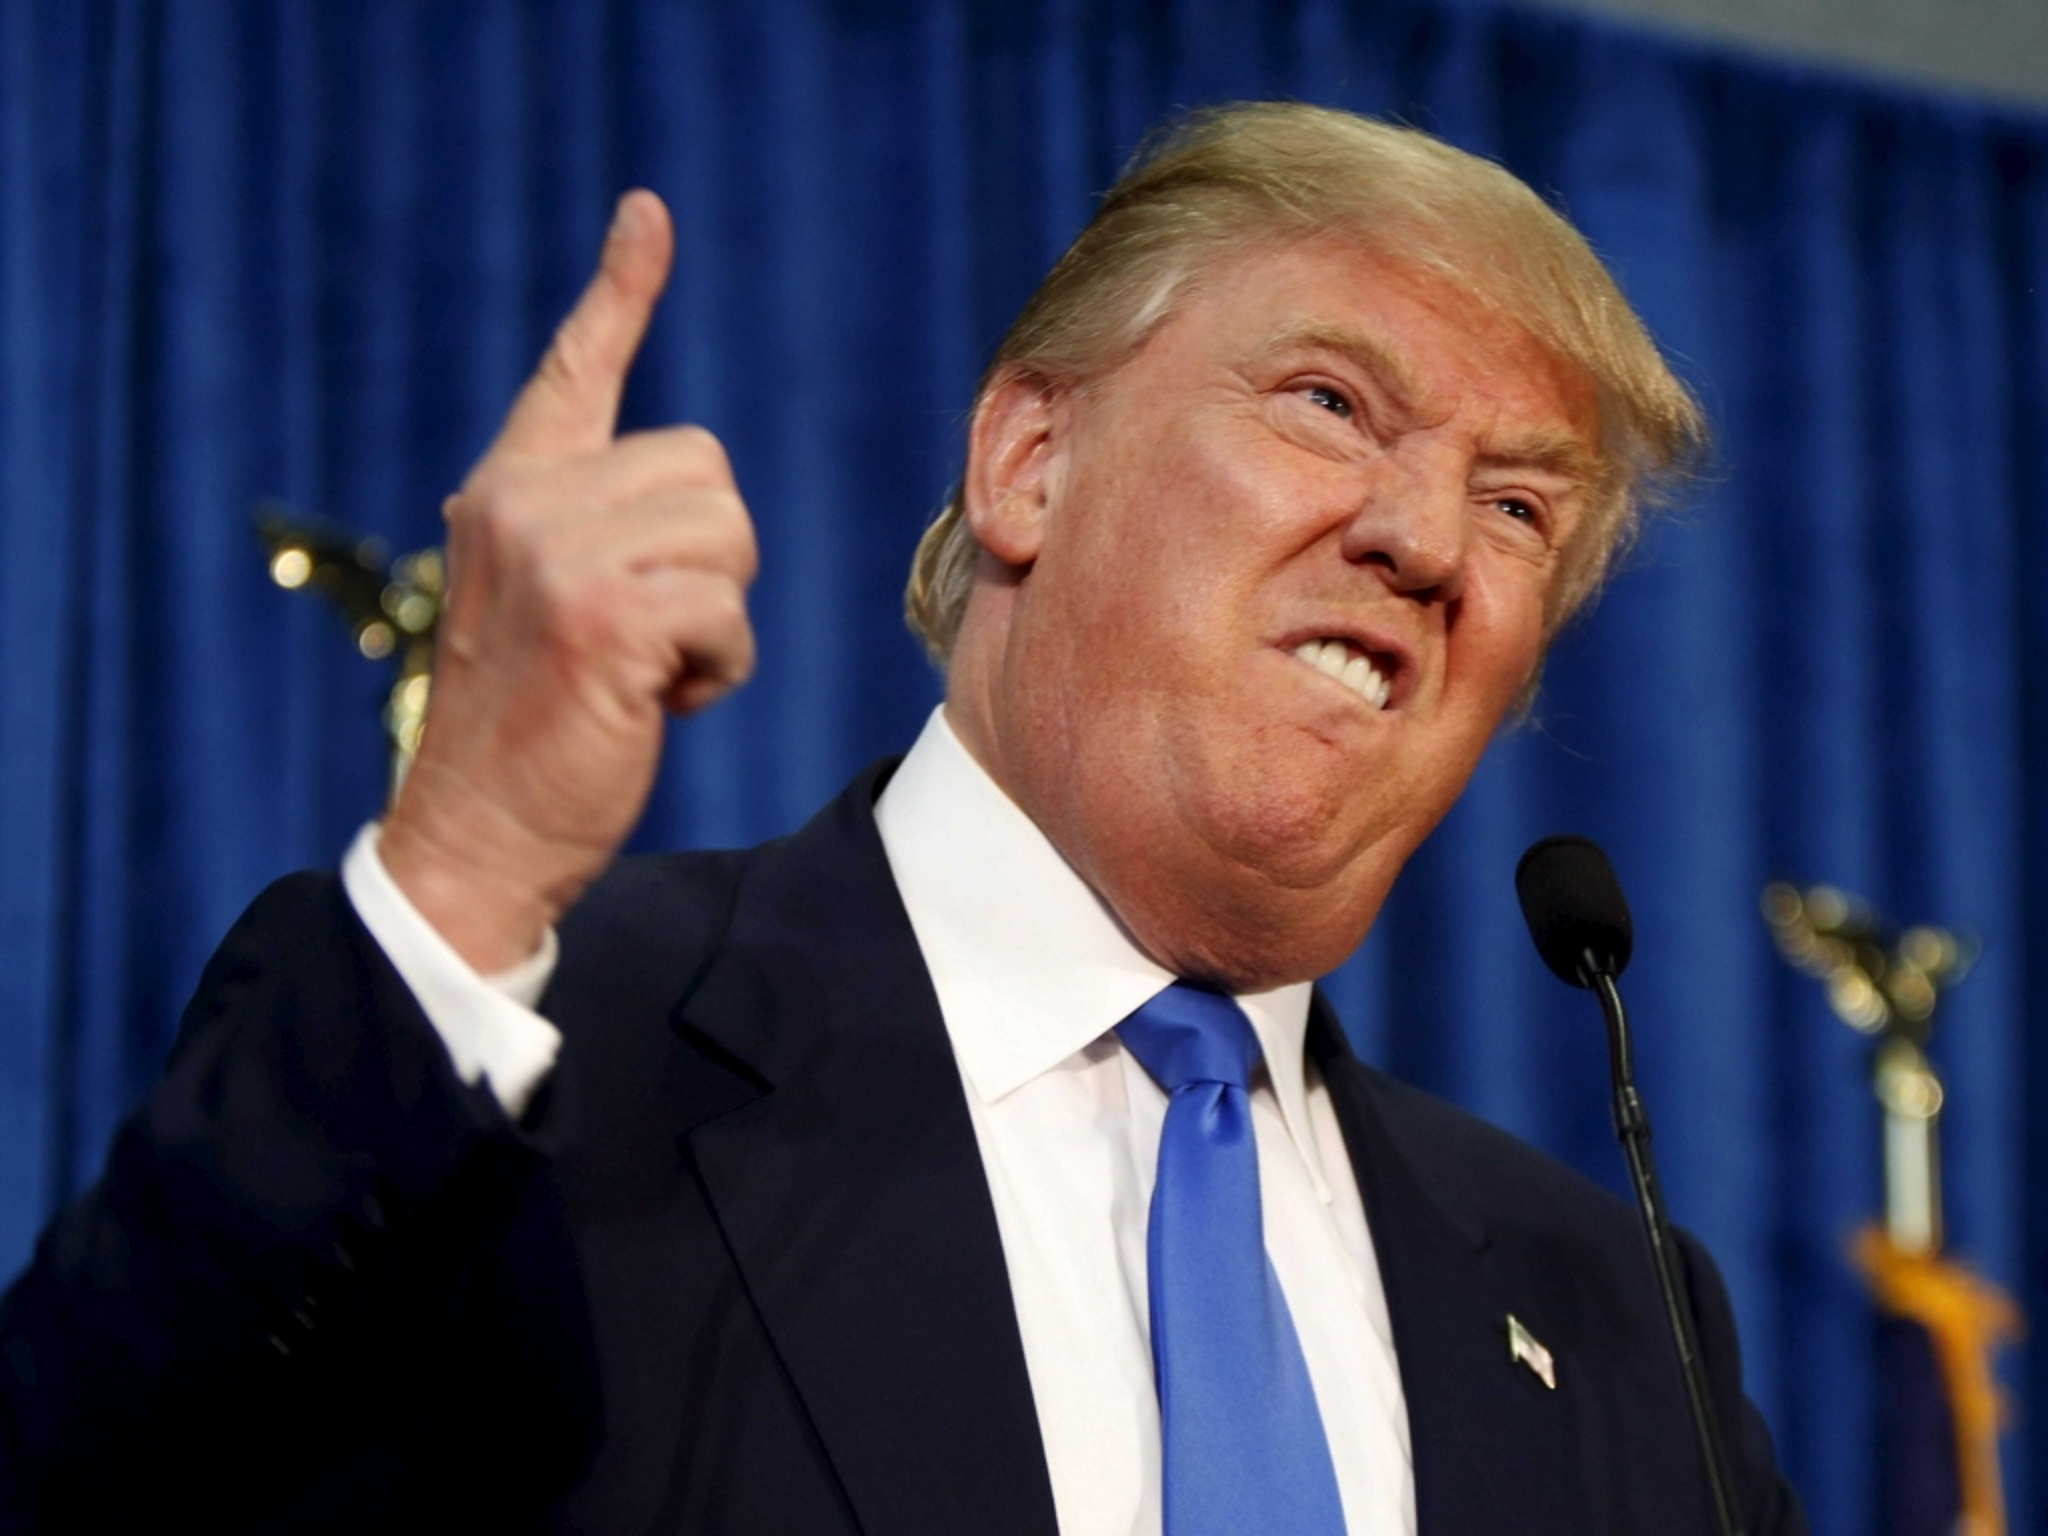
\includegraphics[width=\columnwidth]{trump01.jpg}
%         \caption{左の図}
%         \label{fig:left}
%     \end{subfigure}
%     % 左の図
%     \begin{subfigure}{0.4\columnwidth}
%         \centering
%         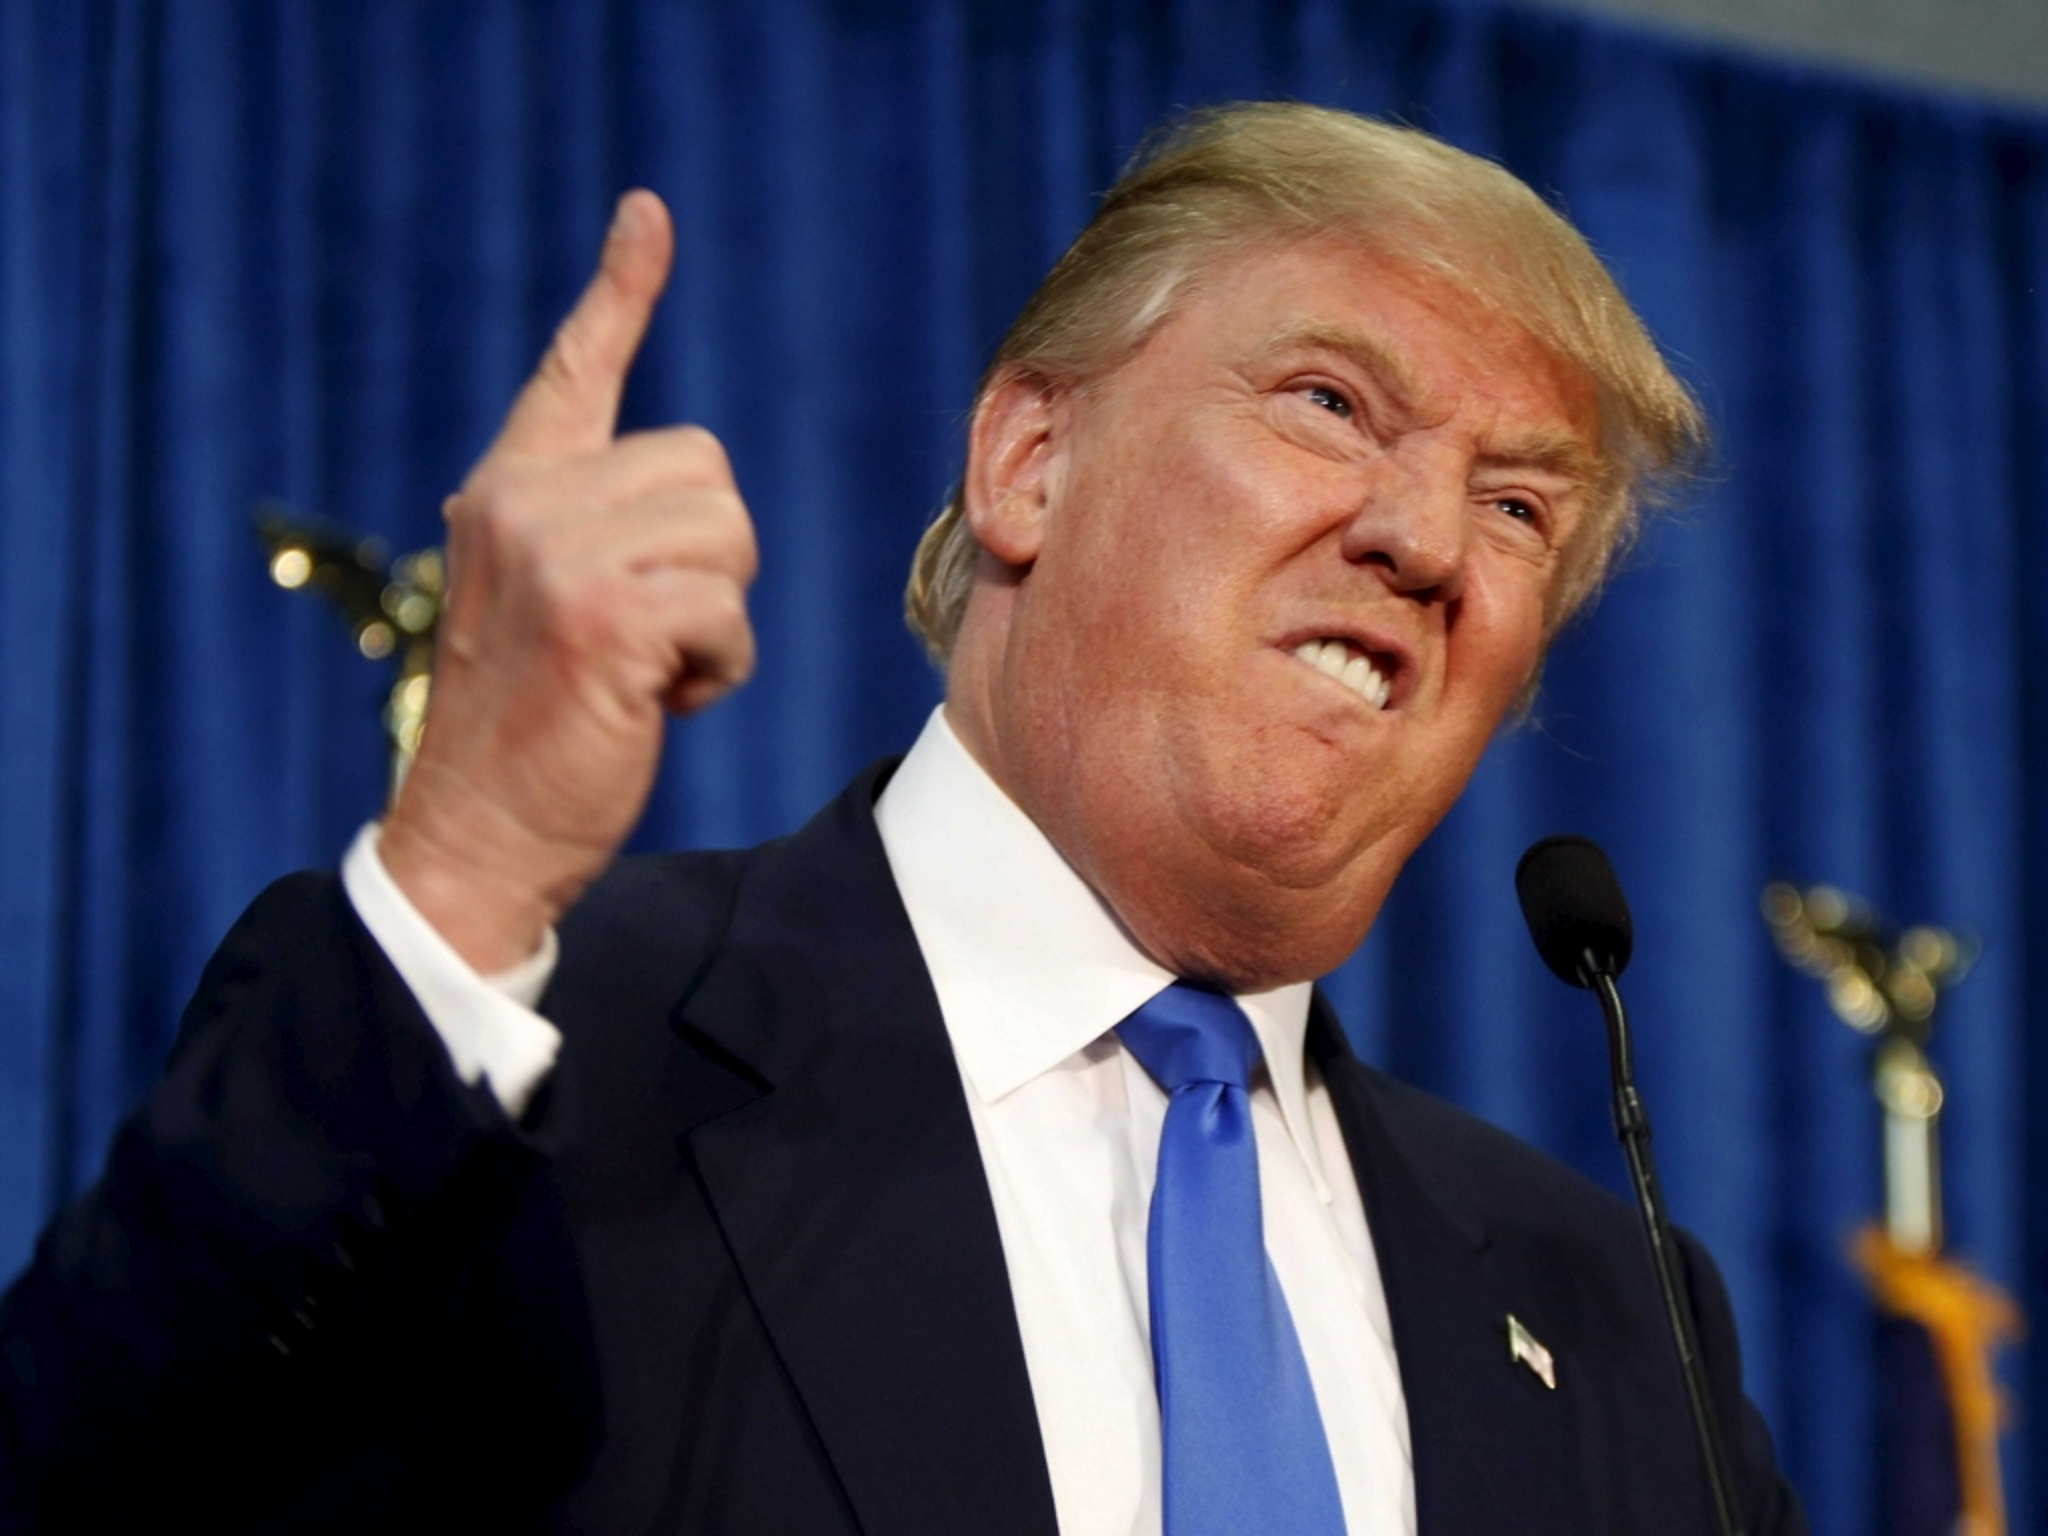
\includegraphics[width=\columnwidth]{trump01.jpg}
%         \caption{右の図}
%         \label{fig:right}
%     \end{subfigure}
%     \\
%     \begin{subfigure}{0.4\columnwidth}
%         \centering
%         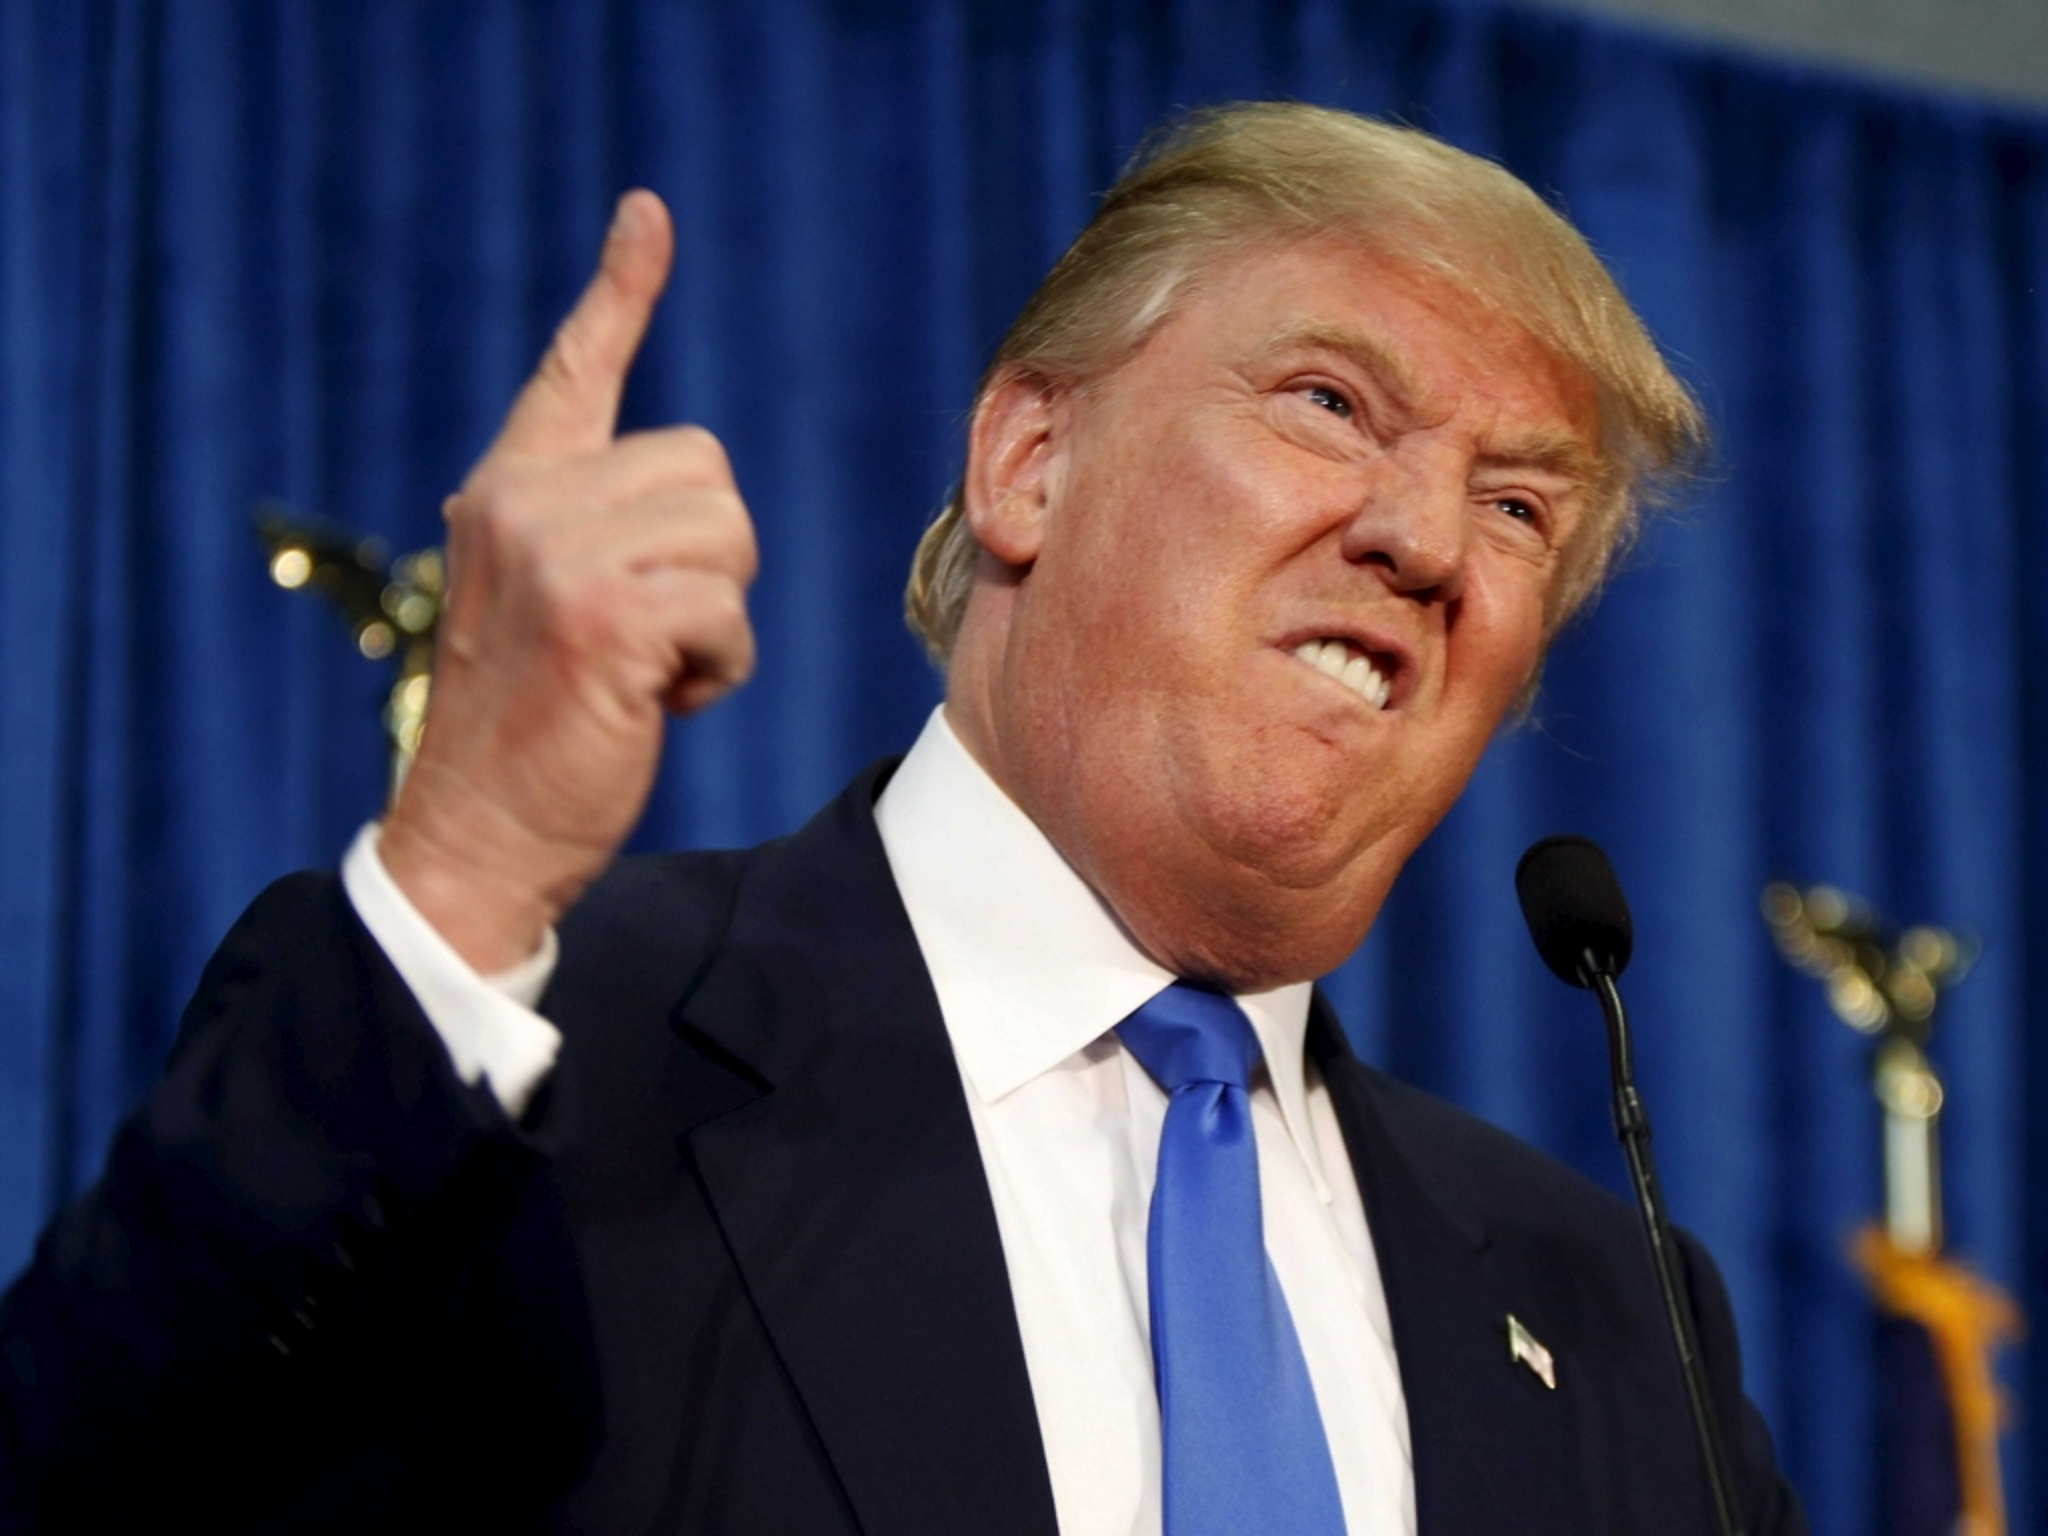
\includegraphics[width=\columnwidth]{trump01.jpg}
%         \caption{左の図}
%         \label{fig:left}
%     \end{subfigure}
%     % 左の図
%     \begin{subfigure}{0.4\columnwidth}
%         \centering
%         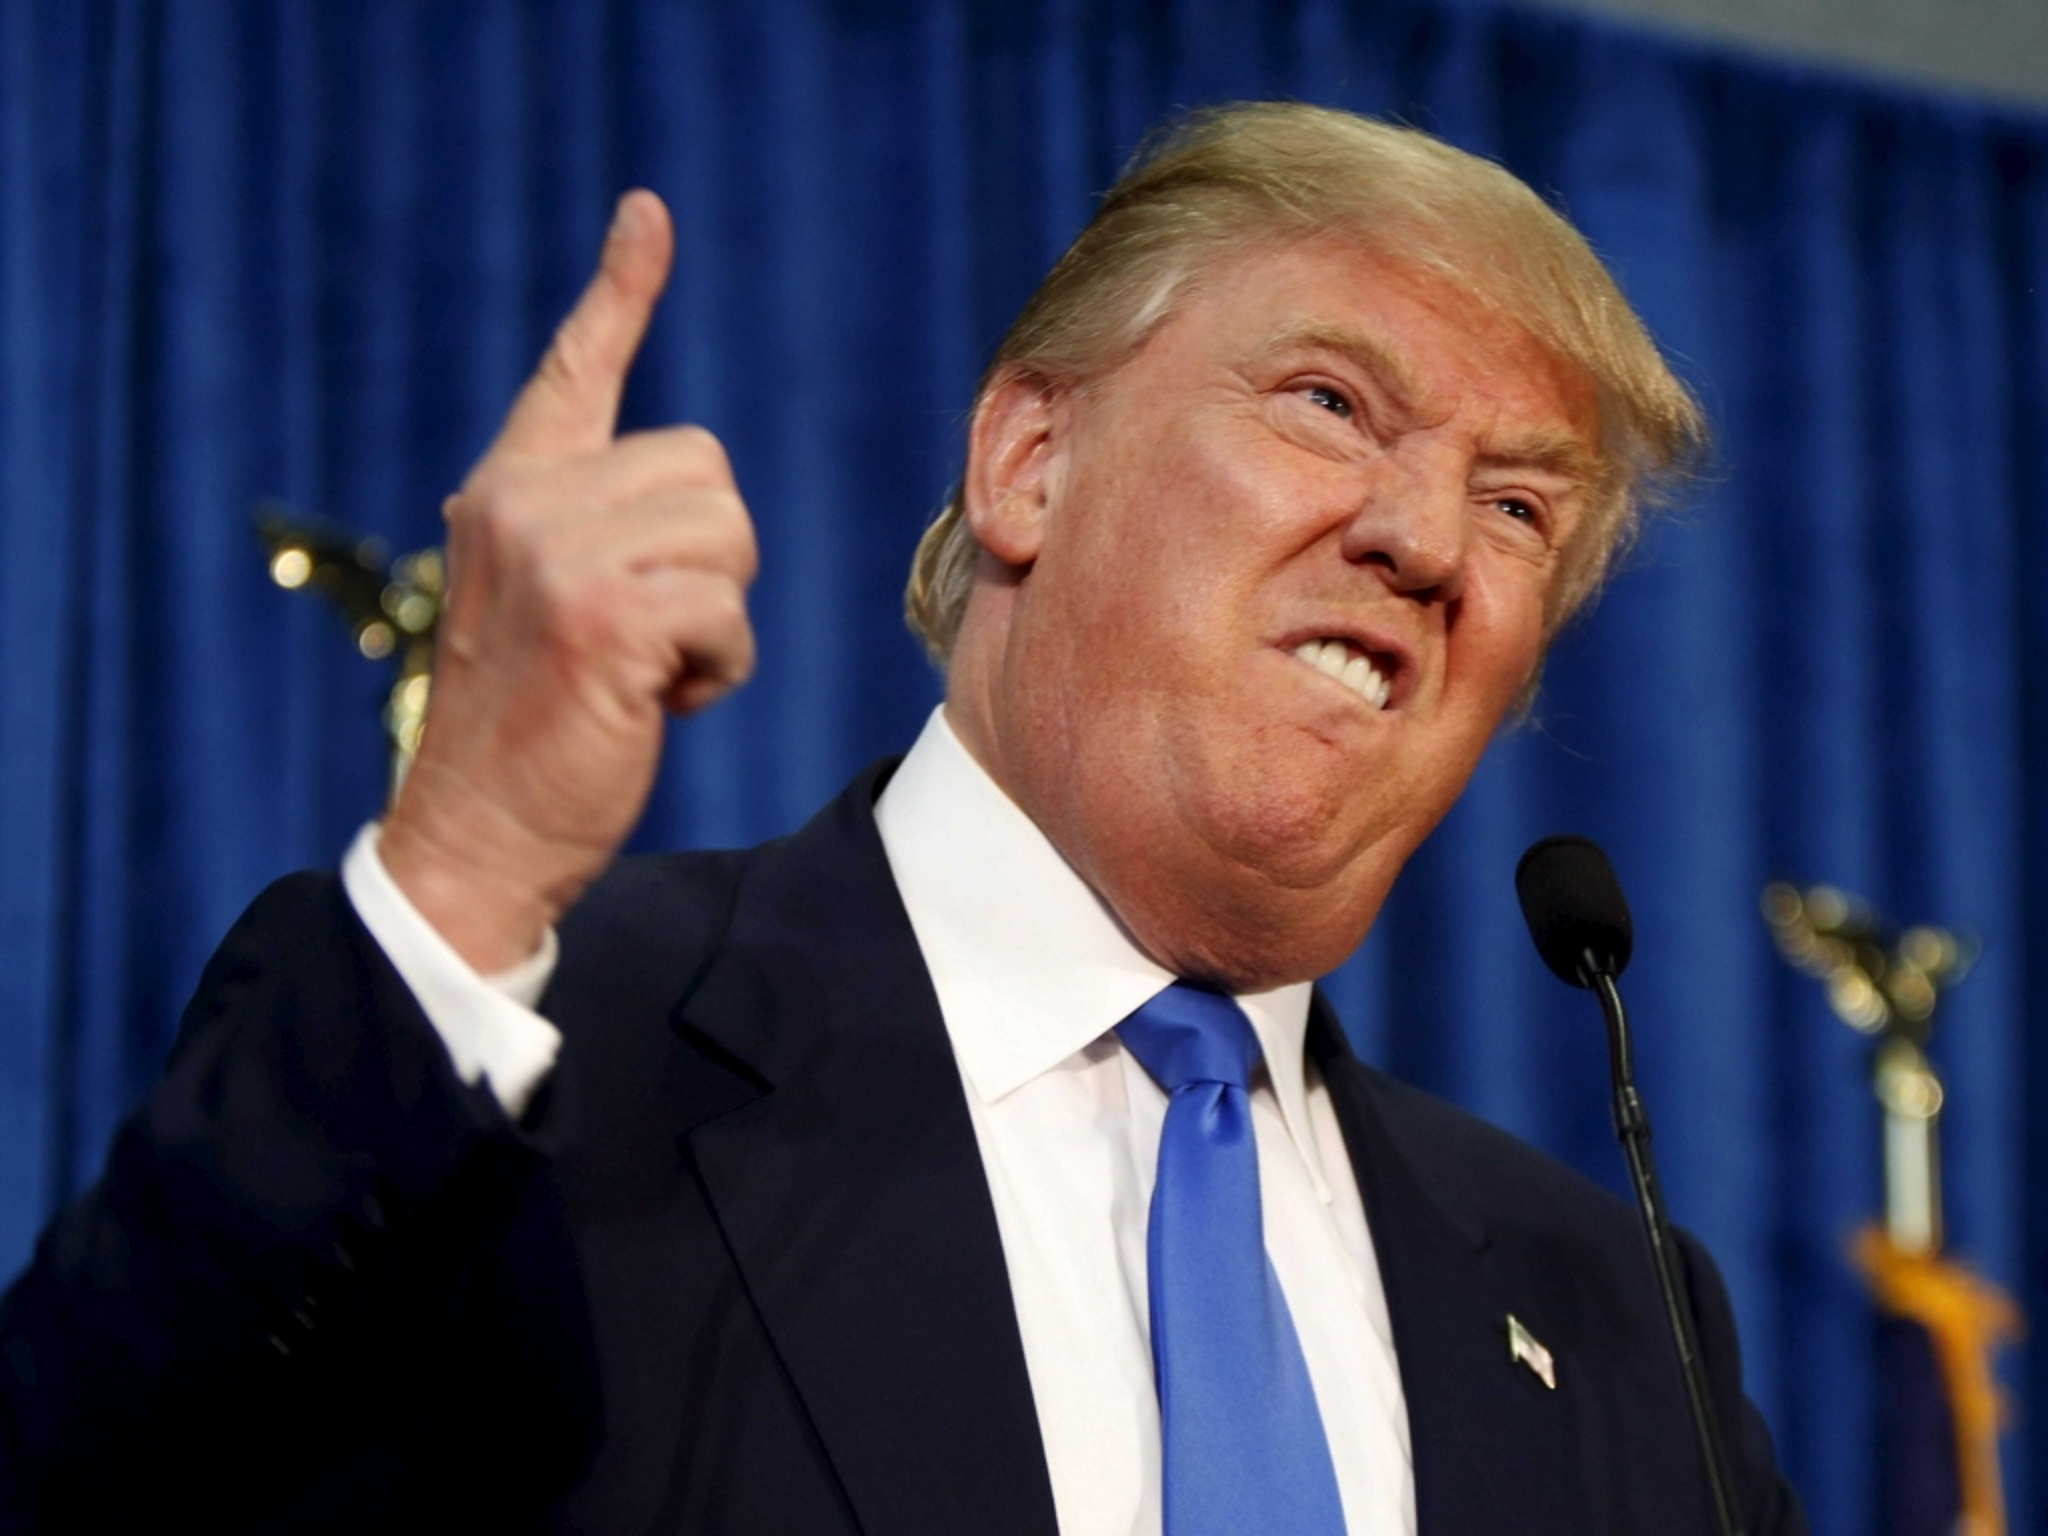
\includegraphics[width=\columnwidth]{trump01.jpg}
%         \caption{右の図}
%         \label{fig:right}
%     \end{subfigure}
%     \caption{左右の図}
% \end{figure}

%\begingroup
% 小数点の桁揃えなど
% ...
% \phantom{ABC}とかくと「ABC」と同サイズの空白が出力されることを使うのが楽
% \pahtom{0}を
% \renewcommand{~}[][]{\phantom{0}}
% とすると便利
%
% 表のキャプション
% \caption[目次用のキャプション]{メインのキャプション}
% 上のコマンドは\begin{}...\end{}の中に書く!!(エラーが出るので)
%
%\endgroup

%\begingroup
%  ...
%\endgroup
